\chapter{Foundations}
\label{ch:foundations}

The main foundations on which this work is based are summarised in this chapter. This includes thermal basics, foundations about thermal modeling and model predictive control (MPC). Note, that in the following all vectors are denoted as bold letters, e.g. \textbf{x}.

\section{Thermal basics}
\label{section:thermalbasics}

There are three different mechanism of heat transfer: Heat conduction, heat convection and heat radiation\cite{.2013}. All of these mechanisms are used for thermal modelling of buildings. For example, conduction is the main part of heat transfer through walls or floors. Convection takes place on the inside and the outside of the building between the walls and the air and radiation is needed for the integration of the impact of the sun, for example.

\subsection{Conduction}
\label{subsection:conduction}

    Conduction means that heat energy is directed in a solid or fluid. Molecules within the solid or fluid have higher energy when the temperature is higher. They transfer the energy to neighbouring molecules with smaller energy. Without a heat source, the temperature difference between a hot and a cold location of the molecules decrease.\cite{Kuchling.2007}
    \newline The equation
    \begin{equation}
    \label{eq:fourier}
        \dot{\textbf{q}} = - \lambda \nabla T
    \end{equation}
    describes the conduction according to Fourier \cite{.2013}. There is $\lambda$ the thermal conductivity with the assumption of being constant and $\dot{\textbf{q}}$ and $T$ represent the specific heat flux and the temperature. The thermal conductivity is dependent on the material, such as concrete, wood or bricks. 
    \newline
    In order to know the heat flux $\dot{Q}$, it is necessary to expand the above equation with the area $A$, the thickness of the conductive medium $d$ and a temperature difference $\Delta T$ assuming one significant direction of the heat flux $\dot{Q}$ to:
    \begin{equation}
    \label{eq:conduction1}
        \dot{Q} = \frac{A\lambda}{d} \Delta T
    \end{equation}
    In terms of buildings, the conductive medium could be walls, floors or roofs.

\subsection{Convection}
\label{subsection:convection}

    Macroscopic movements of a fluid  lead to transport of kinetic energy and enthalpy.this mechanism is called convection. These movements are generated by external forces or by internal forces like balancing the pressure or temperature.\cite{.2013}
    \newline
    Newton's law of cooling describes the convective heat transfer $\dot{Q}$ as 
    \begin{equation}
    \label{eq:newton}
        \dot{Q} = \alpha A (T_w - T_\infty)
    \end{equation}
    with the heat transfer coefficient $\alpha$, especially for building modeling the wall temperature $T_w$ and the environment temperature $T_\infty$ \cite{Griesinger.2019}
    . There are two possibilities to determine the heat transfer coefficient. Both require a temperature difference $\Delta T$ and either a temperature gradient $\partial T/\partial x$ or a heat flux $\dot{Q}$.
    \cite{.2013} 

\subsection{Radiation}
\label{subsection:radiation}

    Every body emits heat radiation to the environment with electromagnetic waves. Especially, heat radiation does not need matter for energy transportation. As shown in the following equation, the temperature $T$ of the body influences highly the heat radiation.\cite{.2013} 
    \begin{equation}
    \label{eq:radiation}
        \dot{q} = \sigma T^4
    \end{equation}
    This correlation applies to a black body, where $\dot{q}$ is a heat flux and $\sigma$ represents the Stefan- Boltzmann coefficient. A black body absorbs all heat radiation with all wave lengths of all directions\cite{Griesinger.2019}. The consideration of a black body is idealized, for the illustration of a real body (see \autoref{eq:realbodyradiation}) the emissivity $\epsilon$ is used. $\epsilon$ is material-dependent and lies between 0 and 1.
    \begin{equation}
    \label{eq:realbodyradiation}
        \dot{q} = \epsilon \sigma T^4
    \end{equation}
    In general, a body absorbs, transmits and reflects radiation with the appropriate coefficients $a$, $\tau$ and $r$. The sum of three coefficients has to be one ($a + \tau + r = 1)$
    \cite{Baehr.2016}.
    In particular, the reflection coefficient is needed for describing the influence of radiation from the environment in building modeling.
    \newline
    The best known source of heat radiation is the sun, which plays an important roll in thermal modeling of buildings. Objectives in the building, such as radiators, also  radiate heat. For example, radiators have equal parts convective and radiative energy transport \cite{Hazyuk.2012}. 
    
\section{Lumped capacitance model}
\label{section:modeling}
For modeling the thermal behavior of buildings, the lumped capacitance model is often used. With this approach, using the electrical analogy, building elements are represented by resistors $R$ and capacitors $C$. \cite{Kramer.2012}

\subsection{Electrical analogy}
\label{electricalanalogy}

    Similar to an electrical network, the potential is represented by the temperature at one node and the heat flux corresponds to the current. We can also use the Ohm's law, which is formulated in the thermal way as:  
     \begin{equation}
    \label{eq:Ohm}
        \dot{Q} = \frac{\Delta T}{R} 
    \end{equation}
    Combining the above equation with \autoref{eq:conduction1} or \autoref{eq:newton}, the thermal resistance $R$ is determined in conductive cases as \cite{Kuchling.2007}:
    \begin{equation}
    \label{eq:r_lambda}
        R_\lambda = \frac{d}{A\lambda}
    \end{equation}
   and in convective cases as\cite{Griesinger.2019}:
    \begin{equation}
        R_\alpha = \frac{1}{\alpha A}
    \end{equation}
    In sum, the thermal resistances $R$ comply with electrical resistors.
    In addiction for modeling thermal networks the thermal capacitance $C$ is needed. It is calculated from the specific heat capacity $c$ multiplied by the mass $m$ ($C=cm$).
    \newline
    For a better explanation of the structure of a thermal network, a simple example is depicted in \autoref{fig:sampleRCnetwork}. It represents a heated wall of a building.
    \begin{figure}[h]
    \centering
    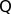
\includegraphics[scale=0.8]{figure/beispiel Netzwerk.png}
    \caption{Sample RC- network}
    \label{fig:sampleRCnetwork}
    \end{figure}
    The heat flux $\dot{Q}$, for example from a radiator, influences the temperature $T_{wall}$, as well as the capacitance $C$. And the temperature $T_{wall}$ affects the temperature inside and outside $T_{inside}$ and $T_{outside}$ with their resistances $R_{\alpha,inside}$ and $R_{\alpha,outside}$. The example shows that all connections in the network influence each other.
    In order to model the dynamics of the wall in differential equations, the Kirchhoff's Current Law is required. It states that the sum of the flowing current to the node is equal to the sum of the flowing current off the node 
    \cite{Kuchling.2007}. 
    Because of the thermal analogy of electrical laws, the current is replaced by the heat flux. The following differential equation results for the node  $T_{wall}$ using Ohm's law ($\dot{Q}=\Delta T/R$) and the relationship $\dot{Q}=C\frac{\partial T}{\partial t}$.     
    \begin{equation}
    \label{eq:sampledifferential}
    C \frac{\partial T_{wall}}{\partial t} = \dot{Q} + \frac{T_{inside}-T{wall}}{R_{\alpha,inside}} - \frac{T_{wall}-T{outside}}{R_{\alpha,outside}}
    \end{equation}
    In \autoref{fig:sampleRCnetwork}, the thermal resistances are serially connected. According to the electrical network, resistances in series are equal to their sum. 
    \begin{equation}
    \label{eq:resistanceseriel}
        R_{sum} = R_{\alpha,inside} + R_{\alpha,outside}
    \end{equation}
    A parallel circuitry has windows and walls in buildings, for example. Here the resistances are calculated according to the following schema:
    \begin{equation}
    \label{eq:resistancesparallel}
        \frac{1}{R_{sum}} = \frac{1}{R_{wall}} + \frac{1}{R_{window}}
    \end{equation}
    In terms of needed more capacitances for describing the thermal model, the summary capacitance is added in a parallel circuitry as: 
    \begin{equation}
    \label{eq:capacityparallel}
         C_{sum} = C_1 + C_2
    \end{equation}
    The serial circuitry of capacitances is calculated as follows:
    \begin{equation}
    \label{eq:capacityseriell}
         \frac{1}{C_{sum}} = \frac{1}{C_1} + \frac{1}{C_2}
    \end{equation}
    
%maschenregel noch erklären?


\section{Model predictive control (MPC)}
\label{section:mpc}

"The idea of model predictive control [...] is [...] to utilize a model of the process in order to predict and optimize the future system behavior"
\cite{Grune.2017}.
Applied to a thermal control of a building with the aim of grid- supporting, a model of the thermal behavior of the building is required to predict the reaction of the system behavior in the next $N$ time steps, called the prediction horizon. Every time step $k$, the current state $\mathbf{x_k}$, the output $\mathbf{y_k}$ is measured and the future system behavior is obtained computation. The computation of the future system behavior may include weather forecast, occupancy schedule  and the optimization of the control signal $\mathbf{u_k}$ over the optimization horizon $\mathbf{u_{k+N}}$. But, only the first calculated control signal is adopt as input for the plant.
Then, the calculation are repeated at every time step. \autoref{fig:sampleMPC} visualises the MPC control loop.
 \begin{figure}[h]
    \centering
    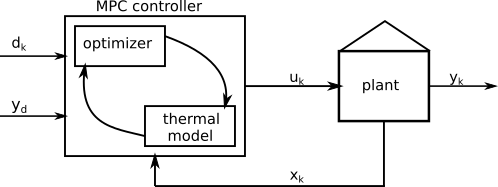
\includegraphics[scale=0.8]{figure/MPC beispiel2.png}
    \caption{MPC structure of the control loop}
    \label{fig:sampleMPC}
    \end{figure}
\newline
Concluded, the MPC is "an iterative online optimization over the predictions"
\cite{Grune.2017} 
compiled by the thermal model of the building. Mathematically explained, the optimizer needs to reduce the following equation according to
\cite{Kouvaritakis.2018}
and
\cite{Oldewurtel.2012}:
\begin{align}
\label{eq:costfunc}
\textrm{Cost function} && minimize \sum_{k=1}^{N-1} c_k(x_k,u_k,y_k)
\end{align}
subject to 
\begin{align*}
\textrm{Current state} && x_0 &=& x \\	
\textrm{Dynamics} && x_{k+1}&=& f(x_k,u_k,d_k)		&&	y_k = g(x_k,u_k,d_k)\\				
\textrm{Constraints} && y_{min}&\leq& y_k \leq y_{max}\\		
\textrm{} && u_{min}&\leq& u_k \leq u_{max}	
\end{align*}
$c_k$ represents the cost function, which is explained in detail in \autoref{subsection:costfunction}
. In terms of building control, $y$ is the internal temperature.
%Störungen noch erklären

\subsection{Cost function}
\label{subsection:costfunction}

    The cost function $c_k$ assigns a cost to the control signal $u_k$ and the current state $x_k$, which is mathematically described in
    \autoref{eq:costfunc}
    , with:
    \begin{equation}
    \label{eq:c_k}
    c_k = (x_k^TQx_k+u_k^TRu_k)
    \end{equation}
    Here $Q$ and $R$ are matrices over which individual elements of the state vector or control signal vector can be weighted differently.  
    \cite{Kouvaritakis.2016}
    %linear, quadratisch, gewichtet 
    %reduziert Zustand, stellsignal

\subsection{Current state}
\label{subsection:currentstate}

    The current state $\mathbf{x_k}$ is a vector of measured state variables of a building. Every prediction starts form this initial state \cite{Oldewurtel.2012}.
    
\subsection{Dynamics}
\label{subsection:dynamics}
    
    The state space formulation (SSF) is an alternative representation of a linear differential equation, which models a physical system. In this work, it is used for the formulation of the thermal model, which is required for the MPC. The SSF consists of the state $\textbf{x}$, the control signal $\textbf{u}$, the disturbances $\textbf{d}$ and the output of the system $\textbf{y}$ represented in \autoref{eq:statespace}. The system matrix is $A$, $B_1$ and $B_2$ are called the input matrices, $C$ is the output matrix, $D_1$ and $D_2$ are the pass- through matrices.  
    \begin{align}
    \label{eq:statespace}
    \dot{\textbf{x}}=A\textbf{x}+B_1\textbf{u}+B_2\textbf{d}\\
    \textbf{y}=C\textbf{x}+D_1\textbf{u}+D_2\textbf{d} \notag
    \end{align}
    In a thermal model of a building, some authors (\cite{Hazyuk.2012}, \cite{Siroky.2011},...) use the state as a vector of some temperatures, the control signal as a signal for the heating system, the disturbances can describe the influence by the weather or occupants and the output of the system contains frequently the temperature inside of the building.
    


\subsection{Constraints}
\label{subsection:constraints}

Dealing with constraints is one of the most important advantages of MPC. Thereby, constraints can be used for the state, the output, and the input. In terms of building control, output constraints and input constraints are reasonable, as mathematically described in the \autoref{eq:costfunc}. That means, the output constraints could be a temperature range, which feels comfortable for occupants. And the constraints for the input are given as minimal (= 0) and maximal values of the possible performances. General, logical and physical ranges are constrained. There are different forms of constraints, but linear constraints are mostly used for MPC, because they simplify the optimization problem. Constraints can also be time dependant. This is beneficial for embedding diverse temperature range during the night and the day or during the working time of occupants, when they are not at home.
\cite{Siroky.2011}
%es gibt harte und weiche constraints. wichtig ist, dass man nicht auf beiden seiten harte constraints einstellt. konvexe Constraints bei bedarf
